\documentclass{article}
\usepackage{cite}
\usepackage{graphicx} % Required for inserting images
\usepackage{float}
\usepackage{listings}
\usepackage{color}

\definecolor{codegreen}{rgb}{0.0, 0.6, 0.0}
\definecolor{codeblue}{rgb}{0.0, 0.0, 0.8}
\definecolor{codegray}{rgb}{0.5, 0.5, 0.5}
\definecolor{codepurple}{rgb}{0.58, 0, 0.82}
\definecolor{backcolour}{rgb}{0.97, 0.97, 0.97}

\lstdefinestyle{lightstyle}{
    backgroundcolor=\color{backcolour},   
    commentstyle=\color{codegreen},
    keywordstyle=\color{codeblue},
    numberstyle=\tiny\color{codegray},
    stringstyle=\color{codepurple},
    basicstyle=\ttfamily\footnotesize,
    breakatwhitespace=false,         
    breaklines=true,                 
    captionpos=b,                    
    keepspaces=true,                 
    numbers=left,                    
    numbersep=5pt,                  
    showspaces=false,                
    showstringspaces=false,
    showtabs=false,                  
    tabsize=2
}

\lstset{style=lightstyle}


\title{Homework 9: Probability and simulation}
\author{Casper Kristiansson}
\date{\today}

\begin{document}

\maketitle

\section{The St. Petersburg paradox}
\subsection{Willingness to pay to enter the game}
In the St. Peterbugs game, the winnings are doubled with each toss of a coin until the first head appears. This means that for the first run if the head appears the payout is 1 and if it appears on the second toss the payout is 2 etc. This means that the probability of the game ending on each toss is \(\frac{1}{2}\). Based on this game we know that the expected value is infinity. This means that any rational person would be willing to pay any finite amount to play.

But here is the problem. Even if the expected value of the game is infinity there are a lot of factors that are not included. In real life being able to gain money on this problem could require a lot of time depending on the initial entry fee.

\subsection{Unrealistic assumptions}
The unrealistic assumption is the infinite amount of trials which is practically impossible. We also assume there are infinite amounts of resources which in this case is payout.

\subsection{Simulation}
We then want to simulate the game. This can easily be done by simply first picking a max payout which I set to the standard value of 10,000,000. We then simulated 50 games where each game consisted of 100,000 rounds.

\begin{figure}[H]
    \centering
    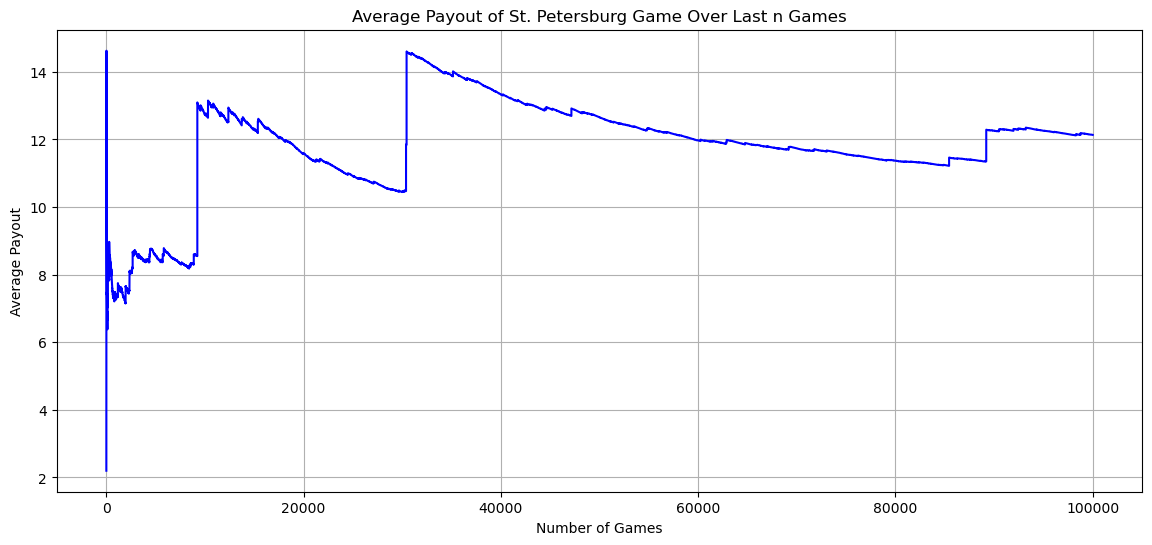
\includegraphics[width=\textwidth]{HW9.png}
    \caption{Average Payout of St. Petersburg Game Over Last n Games}
    \label{fig:graph}
\end{figure}

\subsection{Convergence}
The convergence is a kind of new expected value that we get based on the casino's maximum payout of 10,000,000. As we can see in the graph the expected value converges toward a smaller number which is about 11-12 SEK.

\section{Unusual number of visitors}
If we want to simulate arrival times for the hospital where each patient arrives independently and with a constant probability per time unit we can utilize the Poisson process. As we know the hospital on average gets 300 visitors per day we can use the following formula to calculate the exponential distribution \cite{numpyran14:online}:


\[f(x; \frac{1}{\beta}) = \frac{1}{\beta} \exp\left(-\frac{x}{\beta}\right)\]

We then can using this formula calculate the distribution and plot it.

\begin{figure}[H]
    \centering
    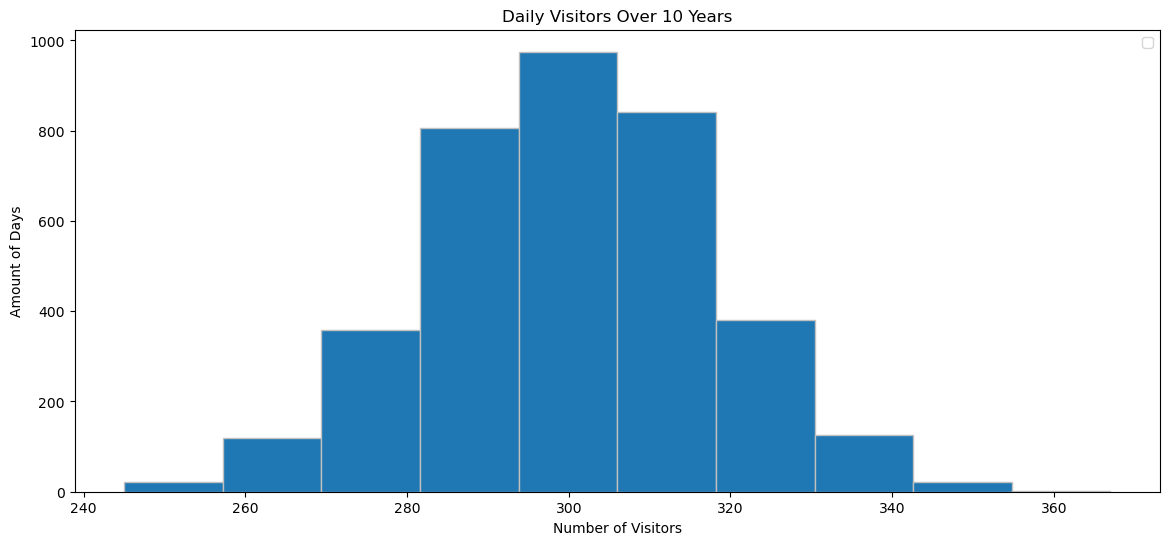
\includegraphics[width=\textwidth]{HW9_2.png}
    \caption{Number of patients per day}
    \label{fig:graph}
\end{figure}

\begin{figure}[H]
    \centering
    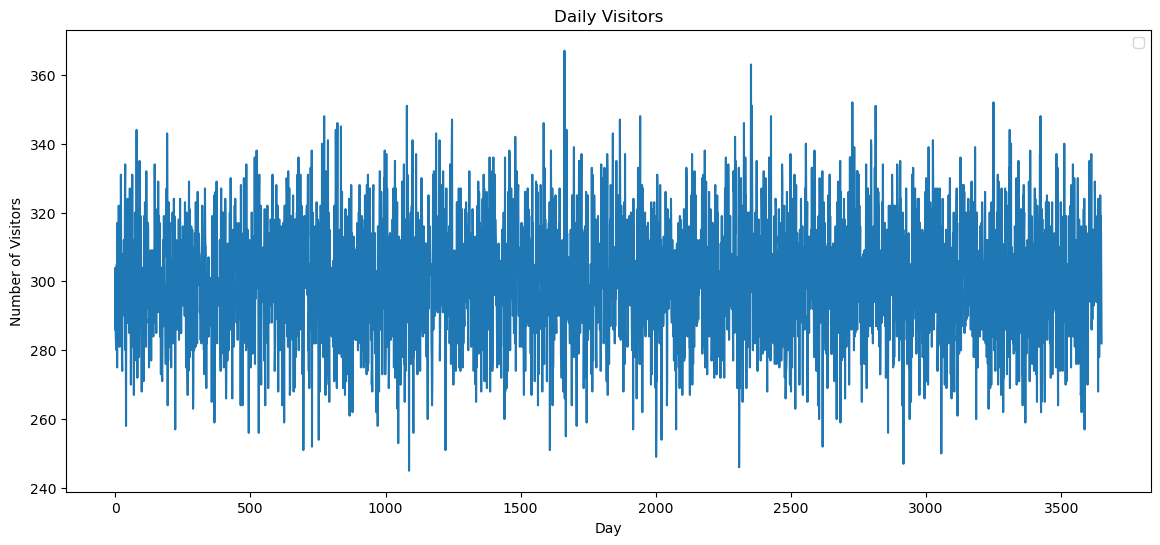
\includegraphics[width=\textwidth]{HW9_3.png}
    \caption{Daily Visitors Over 10 Years}
    \label{fig:graph}
\end{figure}

From the graphs and data, we can see that there were 0 occasions where there were more or equal to 369 visitors.


\appendix

\section{St. Petersburg paradox code}
\begin{lstlisting}[language=Python][H]
max_payout = 10000000
number_of_games = 100000
num_simulations = 50
\end{lstlisting}

\begin{lstlisting}[language=Python][H]
def simulate_game(max_payout):
    payout = 1
    while np.random.rand() > 0.5:
        payout *= 2
        if payout > max_payout:
            return max_payout
    return payout

def run_simulations(n_games, max_payout, num_simulations):
    average_payouts = np.zeros(n_games)
    for _ in range(num_simulations):
        total_payout = 0
        for game in range(1, n_games + 1):
            total_payout += simulate_game(max_payout)
            average_payouts[game - 1] += total_payout / game
    return average_payouts / num_simulations
\end{lstlisting}

\begin{lstlisting}[language=Python][H]
average_payouts = run_simulations(number_of_games, max_payout, num_simulations)

plt.figure(figsize=(14, 6))
plt.plot(range(1, len(average_payouts) + 1), average_payouts)
plt.xlabel('Number of Games')
plt.ylabel('Average Payout')
plt.title('Average Payout of St. Petersburg Game Over...')
plt.grid(True)
plt.show()
\end{lstlisting}



\section{Unusual number of visitors}

\begin{lstlisting}[language=Python][H]
lambda_rate = 300
total_days = 365 * 10
\end{lstlisting}

\begin{lstlisting}[language=Python][H]
def simulate_day(lambda_rate):
    time = 0
    visitors = 0
    while time < 1:
        time += np.random.exponential(1 / lambda_rate)
        if time < 1:
            visitors += 1
    return visitors

def simulations(lambda_rate, total_days):
    visitors = []
    for _ in range(total_days):
        visitors.append(simulate_day(lambda_rate))
    
    return visitors
\end{lstlisting}

\begin{lstlisting}[language=Python][H]
daily_visitors = simulations(lambda_rate, total_days)

plt.figure(figsize=(14, 6))
plt.plot(daily_visitors)
plt.xlabel('Day')
plt.ylabel('Number of Visitors')
plt.title('Daily Visitors')
plt.legend()
plt.show()

plt.figure(figsize=(14, 6))
plt.hist(daily_visitors, edgecolor='silver')
plt.xlabel('Number of Visitors')
plt.ylabel('Amount of Days')
plt.title('Daily Visitors Over 10 Years')
plt.legend()
plt.show()
\end{lstlisting}

\bibliographystyle{IEEEtran}
\bibliography{main}

\end{document}
